\documentclass{article}
\usepackage{amsmath}
\usepackage{graphicx}
\usepackage{longtable}
\usepackage{amsfonts}
\usepackage{listings}
\usepackage{float}
\usepackage{tabularx}
\usepackage{array}
\title{Demostración de NP-Completitud de 3D-Matching}
\author{Francisco Vicente Suárez Bellón}
\date{Septiembre de 2024}

\begin{document}
\maketitle
\newpage
\tableofcontents %generar índice
\newpage

\section{Descripción del problema}
\begin{enumerate}
    \item Sea $M \subseteq  W \times  X \times Y$
    \item $W \cap Y \cap X = \emptyset $(disjuntos)
    \item $|W|=|X|=|Y|=q$
    
\end{enumerate}
Se quiere conocer si existe un matching en M, osea un $M^{'}\subseteq M$ tal que:
\begin{enumerate}
    \item $|M^{'}|=q$
    \item Todos los elementos de $W \cup X \cup Y$ están en algún triplo de $M^{'}$ sin repetir ninguno.
\end{enumerate}

%Foto sobre ejemplo posible 3DM
\begin{figure}[H]
    \centering
    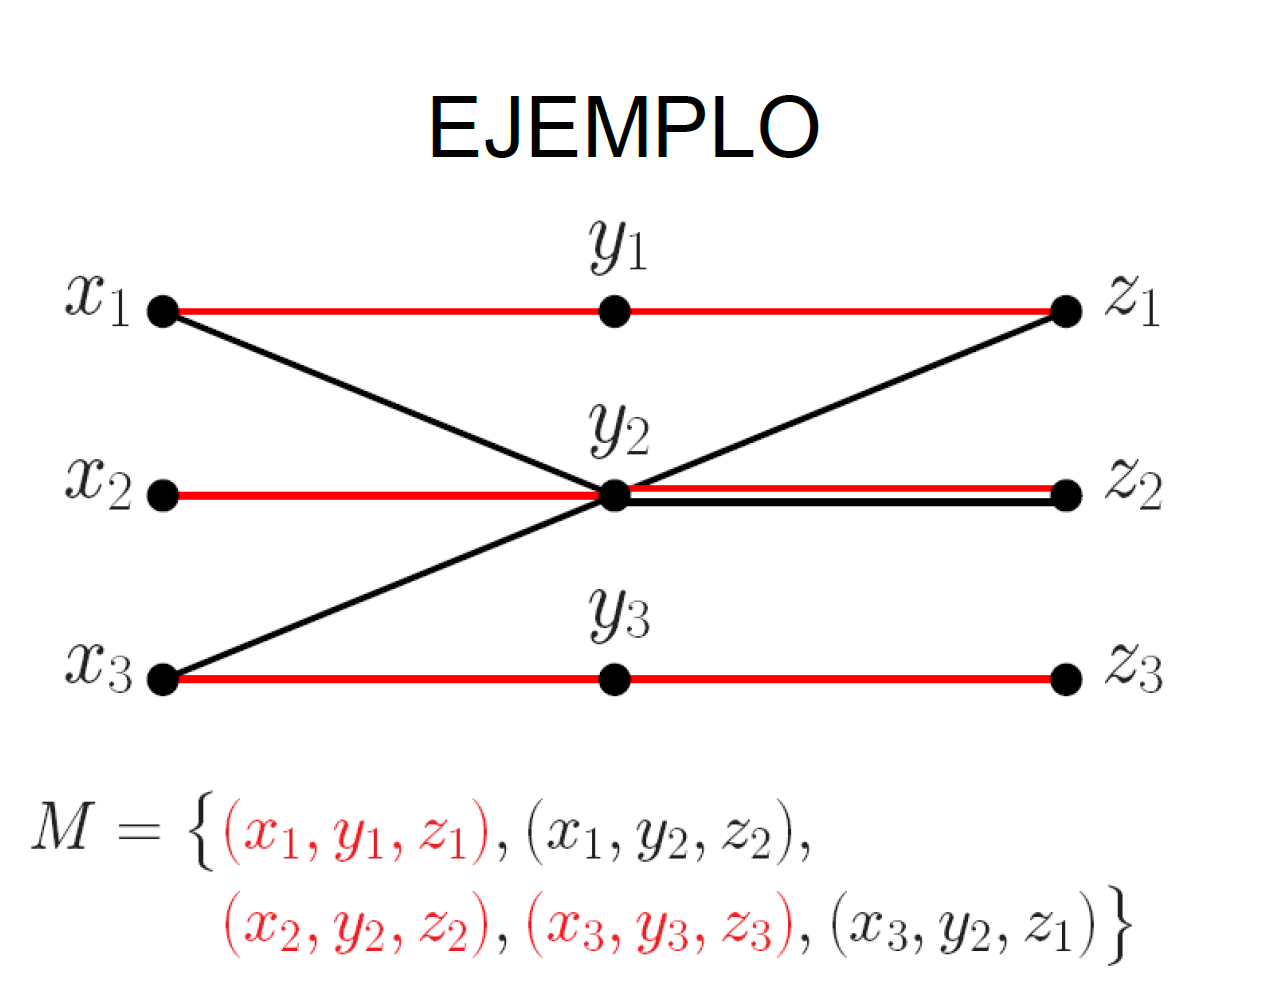
\includegraphics[width=0.5\textwidth]{photos/3_DM_example_1.png}
    \caption{Ejemplo de posible entrada}
    \label{fig:etiqueta}
\end{figure}


\newpage
\section{Análisis del problema}
Aunque el problema para 2-Matching si tiene solución polinomial mediante una red de flujo,
las restricciones de preferencia de cada elemento de la tupla con las otras duplas posibles no hacen posible su codificación mediante esta técnica.

Inicialmente la misma estructura del problema parece indicar que su solución pasa en el peor de los casos con comprobar todas las
posibles soluciones, dado que conformar un triplo puede condicionar que otro no sea formado y no puede ser conocido de antemano. 
Por tanto se procede a examinar si este problema es NP-Completo.
\section{Demostración de NP-Completitud}
\textbf{Pasos Principales:}
\begin{enumerate}
    \item Demostrar que 3DM $\in$ NP
    \item Seleccionar un problema el cual se NP-Completo para hacer la reducción
    \item Construir la transformacion del problema hacia 3DM
    \item Demostrar que la transformación es en tiempo polinomial
\end{enumerate}
\newpage

\section{3DM es NP}
Dada una instancia de (M, X , Y, M) del 3DM se construye un algoritmo no determinista que genere una solución de 
$|W|$ triplos y compruebe en un  tiempo polinomial que no hay dos tercetas con elementos comunes.

\section{Problema NP-Completo para hacer la reducción}
Para ello elegimos el 3-SAT
\subsection{Definición de 3-SAT}
\begin{enumerate}
    \item Sea un conjunto de $m$ cláusulas $C={c_1, \dots , c_m}$ con $|c_i|=3$ $1 \leq i \leq m$
    \item Sobre un conjunto finito de $n$ variables booleanes $U={u_1, \dots, u_n}$
    
\end{enumerate}
Se responde si existe alguna asignación válida de $U$ que satisfaga todas las cláusulas

%Ejemplo como se hará la reducción
\begin{figure}[H]
    \centering
    \includegraphics[width=0.5\textwidth]{photos/ejemplo_como_se_hará_reduccion.png}
    \caption{Reducciíon de 3-SAT a 3-DM}
    \label{fig:etiqueta}
\end{figure}

\subsection{Traducción desde 3-SAT hacia 3-DM}

\begin{table}[h!]
    \centering
    \begin{tabularx}{\textwidth}{|X|X|}
        \hline
        \textbf{3-Sat} & \textbf{3-DM} \\
        \hline
        Variables: $u_1, \ldots, u_n$ & Variables: $u_i(j), b_i(j), S_x(j), G_y(j)$ \\
        \hline
        Literales: $u_1, \lnot u_1$ & Variables: $u_i, \lnot u_{i}(j)$ \\
        \hline
        Cláusulas: $C_{j}=(u_1,\lnot u_2,u_3)$ & Tercetas: $C_{j}\{\left(u_1(j), S_{x}(j), S_{y}(j)\right), \left(\lnot u_2(j), S_{x}(j), S_{y}(j)\right), \left(u_3, S_{x}(j), S_{y}(j)\right)\}$ \\
        \hline
    \end{tabularx}
    \caption{Comparación entre 3-Sat y 3-DM}
\end{table}

\subsection{Definición de los Componentes}
Para realizar la demostración contruiremos unas abstracciones llamadas componentes de las cuales hay 3 tipos:
\begin{enumerate}
    \item Ternas de asignación
    \item Ternas de satisfacción
    \item Ternas de recolección
    
\end{enumerate}

\subsubsection{Definición de las Ternas de asignación}
\begin{enumerate}
    \item Para cada variable $u_i \in U$ se introduce una componente $T_i$
     \begin{enumerate}
        \item $T_i$ depende del número de cláusulas de $m$ en $C$
        
     \end{enumerate}
     \item La estructura del $T_i$
     \begin{enumerate}
        \item Elementos internos:
        $a_i[j]\in X$,  $b_i[j] \in Y$ , $1 \leq j \leq m$ \\
        No van a pertener a otras ternas de otro $T_i$.
        \item Elementos externos:
        \item $\lnot u_i[j] \in W$ ,  $1 \leq j \leq m$\\
        Pueden pertenecer a otras ternas.

     \end{enumerate}
     \item El literal $u_i$ en 3-SAT puede ser usado en varias cláusula, en el 3-DM debemos tener muchas $m$ copias de $u_i$
     %Ejemplo terna de asignación
     \begin{figure}[H]
        \centering
        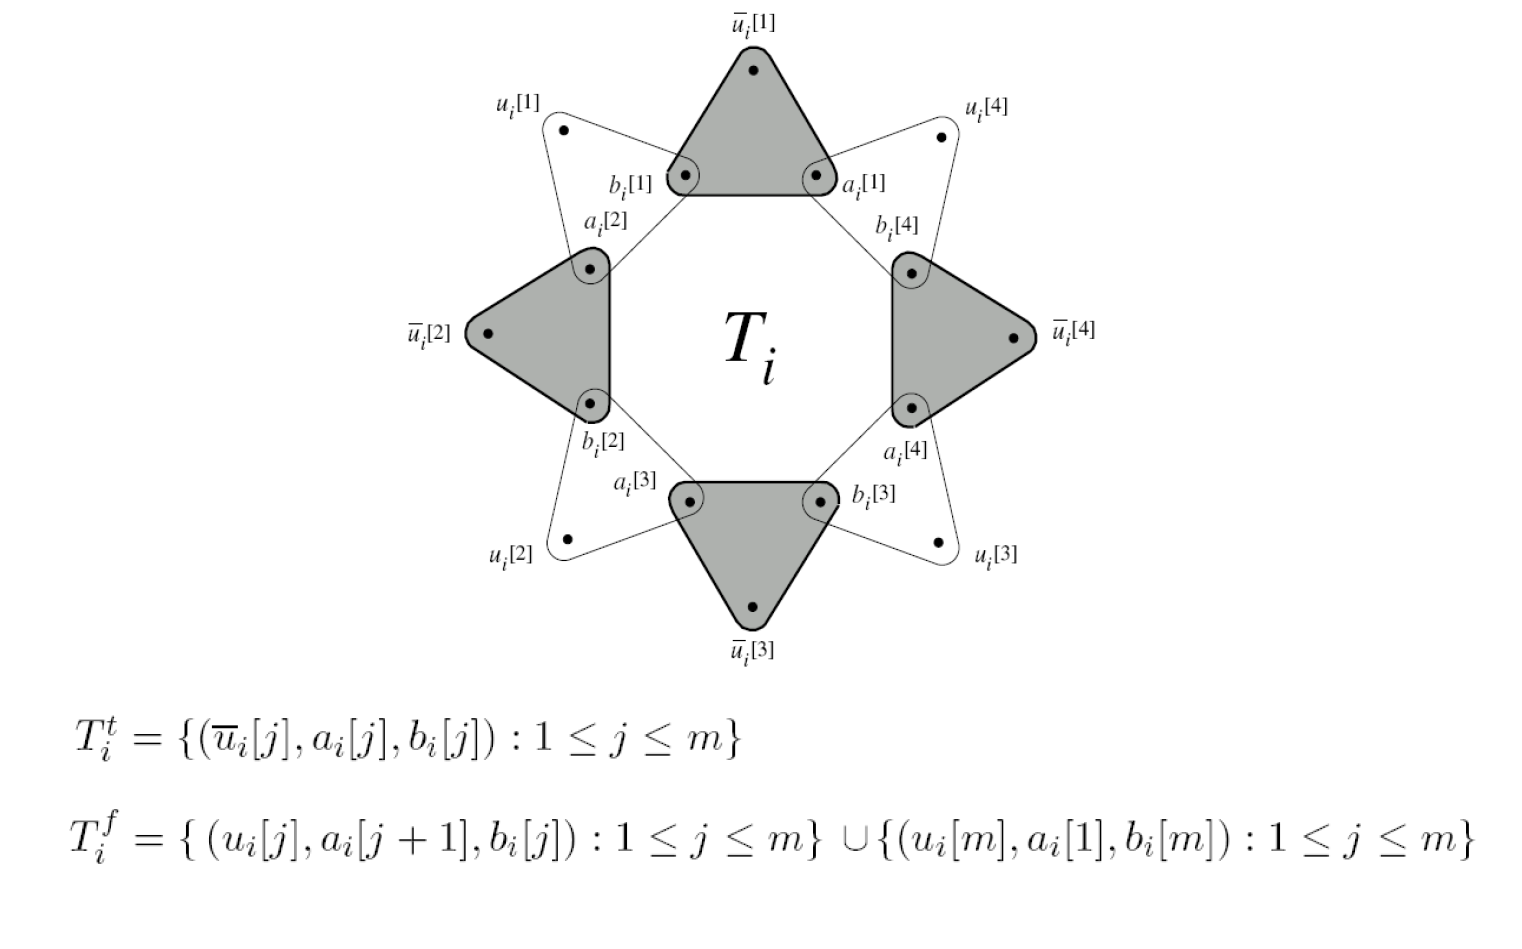
\includegraphics[width=0.5\textwidth]{photos/ejemplo_terna_asignacion.png}
        \caption{Ejemplo terna de asignación}
        \label{fig:etiqueta}


    \end{figure}
    
    \item Si ningún elemento interno de la componente $T_i$ aparece en otra $T_h$
con $h \neq i$
    \item $M^{'}$ será matching con $m$ elementos de $T_i$
    %Ejeplo para cuando $u_i = False $ y $u_i = True$
    \begin{figure}[H]
        \centering
        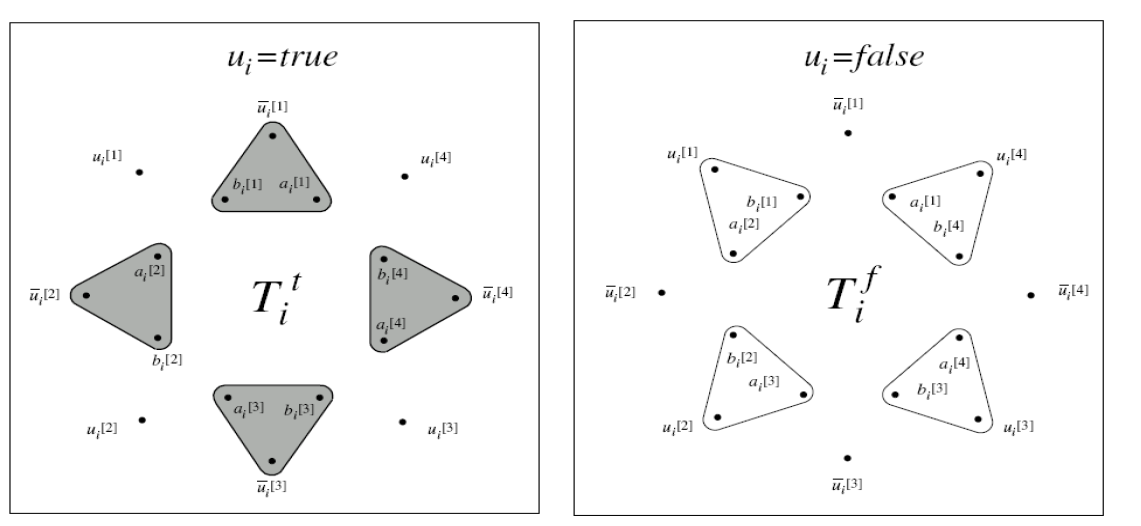
\includegraphics[width=0.5\textwidth]{photos/ternas_asignacion_con_uifalse_ui_true.png}
        \caption{Ejeplo para cuando $u_i = False $ y $u_i = True$}
        \label{fig:etiqueta}
    \end{figure}

    \item Si $u_i =True$ se elegirá como $M^{'}$ las ternas en gris, dejando libre el resto para poder utilizarlas en la contrucción del resto de componentes
    
\end{enumerate}

 
\subsubsection{Definición ternas de satisfacción}
Para cada cláusula $c_j \in C$ introducimos una componente $C_j$

La estructura será la siguiente:
\begin{itemize}
    \item Elementos internos: $s_x[j] \in X$, $s_y[j] \in Y $, $1 \leq j \leq m$
    \item Elementos externos: $u_i[j], \lnot u_i[j] \in W $,$1 \leq j \leq m$
    
\end{itemize}

Donde tendremos que $C_j=\{(u_i[j],s_x[j],s_y[j]):\text{si el literal $u_i \in c_j$  } \cup \text{ } (\lnot u_i[j],s_x[j],s_y[j]):\text{si el literal $\lnot u_i \in c_j$}\} $

\begin{figure}[H]
    \centering
    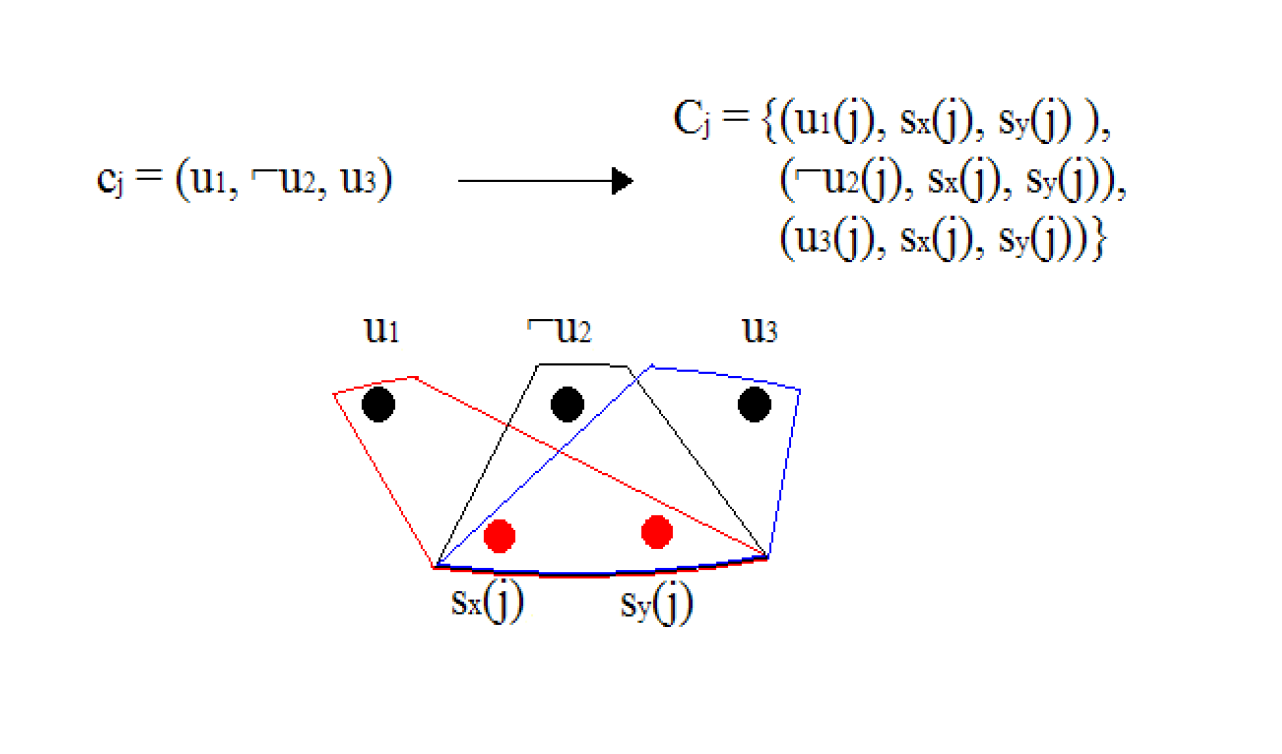
\includegraphics[width=0.5\textwidth]{photos/ejemplo_componente_satisfaccion.png}
    \caption{Ejemplo de la componente de satisfacción}
    \label{fig:etiqueta}
\end{figure}

Además se tiene que cumplir que:
Para cualquier matching $M^{'} \subseteq M$ debe contener una terna de $C_j$ para emparejar los elementos internos 
$s_x[j]$ y $s_y[j]$ bajo esta condición:
\begin{itemize}
    \item $s_x[j]$ y $s_y[j]$ pueden estar emparejados, ssi, al menos uno de los literales $u_i$ de $c_j$ no ha sido emparejado en alguna componente de asignación
$T_i$,$(T_i \cap M^{'})$
\item Si tenemos una 3-SAT instancia factible, entonces las variables $s_x[j]$ y $s_y[j]$ pueden ser emparejadas.
\item Si tenemos una 3-SAT instancia no factible, entonces las variables $s_x[j]$ y $s_y[j]$ no pueden ser emparejadas.
\end{itemize} 

\subsection{Componentes de recolección (Garbage collection)}
Al existir muchos $u_i[j]$ que no se emparejan con componentes de asignación ni con los componentes de satisfacción
Introducimos $m(n-1)$ nuevas varibles.
$g_x[k] \in X, g_y \in Y : 1\leq k \leq m(n-1)$ dado que
hay $m \times n$ variables dse asignación $u$ sin emparejar después de calcularr las tercetas de asignación.Además si todas las $m$ cláusulas
se satisfacen se han emparejado $m$ variables, por lo tanto quedan sin emparejar $(m \times n) - m = m(n-1)$


Finalmente cada pareja $(g_x[k], g_y[k])$ se enlazará con una única variable $u_i[j]$ o $\lnot u_i[j]$ que no estén en las tercetas que se han formado con las componentes anteriores:

%Ejemplo componente recolección
\begin{figure}[H]
    \centering
    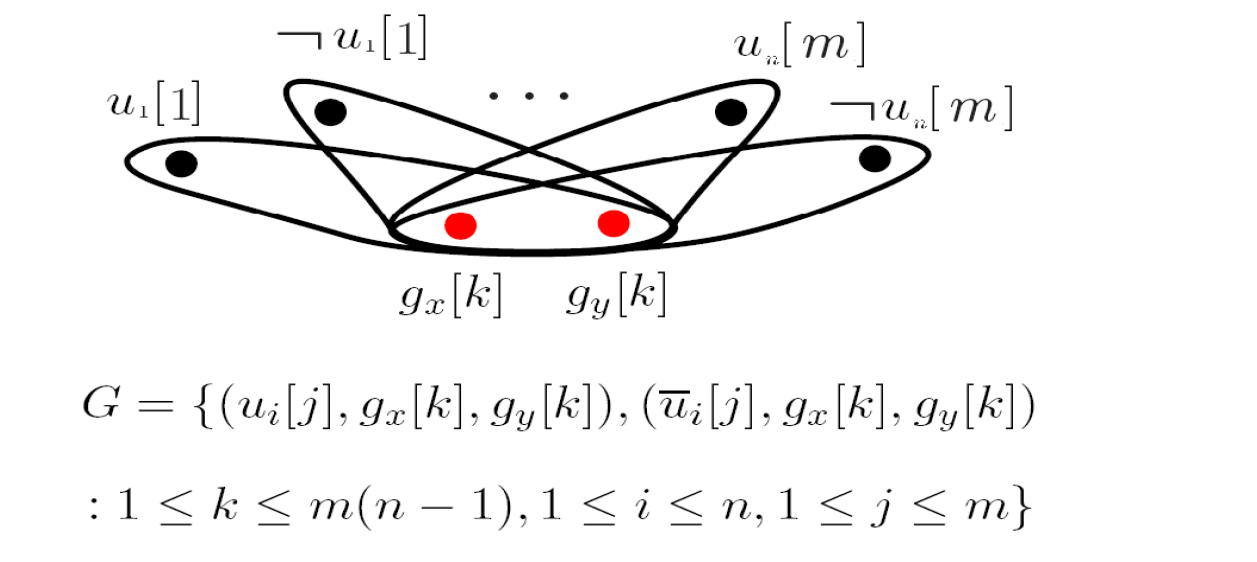
\includegraphics[width=0.5\textwidth]{photos/Ejemplo_garbage_componente.png}
    \caption{Ejemplo componente de recolección}
    \label{fig:etiqueta}
\end{figure}

$W = \left\lbrace u_{i}\left[j\right], \lnot u_{i}\left[j\right] : 1 \leq i \leq n, 1 \leq j \leq m \right\rbrace$

$\linebreak$
\begin{itemize}
    \item $X = A \cup S_{x} \cup G_{x} \quad (2mn)$

\begin{itemize}
    
    \item $A = \left\lbrace a_{i}\left[j\right] : 1 \leq i \leq n, 1 \leq j \leq m \right\rbrace $
    \item \( S_{x} = \left\lbrace s_{x}\left[j\right] : 1 \leq j \leq m \right\rbrace \)
    \item \( G_{x} = \left\lbrace g_{x}\left[j\right] : 1 \leq j \leq m(n-1) \right\rbrace \)
\end{itemize}


\item $Y = B \cap S_{y} \cup G_{y} \quad (2mn)$

\begin{itemize}
    \item $ B = \left\lbrace b_{i}\left[j\right] : 1 \leq i \leq n, 1 \leq j \leq m \right\rbrace $
    \item  $S_{y} = \left\lbrace s_{y}\left[j\right] : 1 \leq j \leq m \right\rbrace $
    \item \( G_{y} = \left\lbrace g_{y}\left[j\right] : 1 \leq j \leq m(n-1) \right\rbrace \)
\end{itemize}

 \item \( M = \bigcup_{i=1}^{n} T_i \cup \bigcup_{j=1}^{m} C_j \cup G. \) 
\( 2mn + 3m + 2m^2n(n-1) \)
\end{itemize}





\begin{tabular}{|c|c|}
    \hline
    \textbf{Significado} & \textbf{Enumeración} \\ \hline
    Cantidad de variables en $<U,C>$ & $n$ \\ \hline
    Cantidad de cláusulas en $<U,C>$ & $m$ \\ \hline
    Cantidad de componentes de \textbf{asignación} triple en $M$ & $2mn$ \\ \hline
    Cantidad de componentes de \textbf{asignación*} triple en $M^`$ & $mn$ \\ \hline
    Cantidad de componentes de \textbf{satisfacción} triple en $M$ & $3m$ \\ \hline
    Cantidad de componentes de \textbf{satisfacción} triple en $M^`$ & $m$ \\ \hline
    Cantidad de componentes \textbf{recolección} en $M$ & $2m^2n(n-1)$ \\ \hline
    Cantidad de componentes \textbf{recolección} en $M^`$ & $m(n-1)$ \\ \hline
    Cardinalidad del emparejamiento perfecto & $2mn$ \\ \hline
    Cardinalidad de $M$ & $2mn=3m=2m^2n(n-1)$ \\ \hline
\end{tabular}

\subsection{Ejemplo de $X,Y,W$}

\begin{figure}[H]
    \centering
    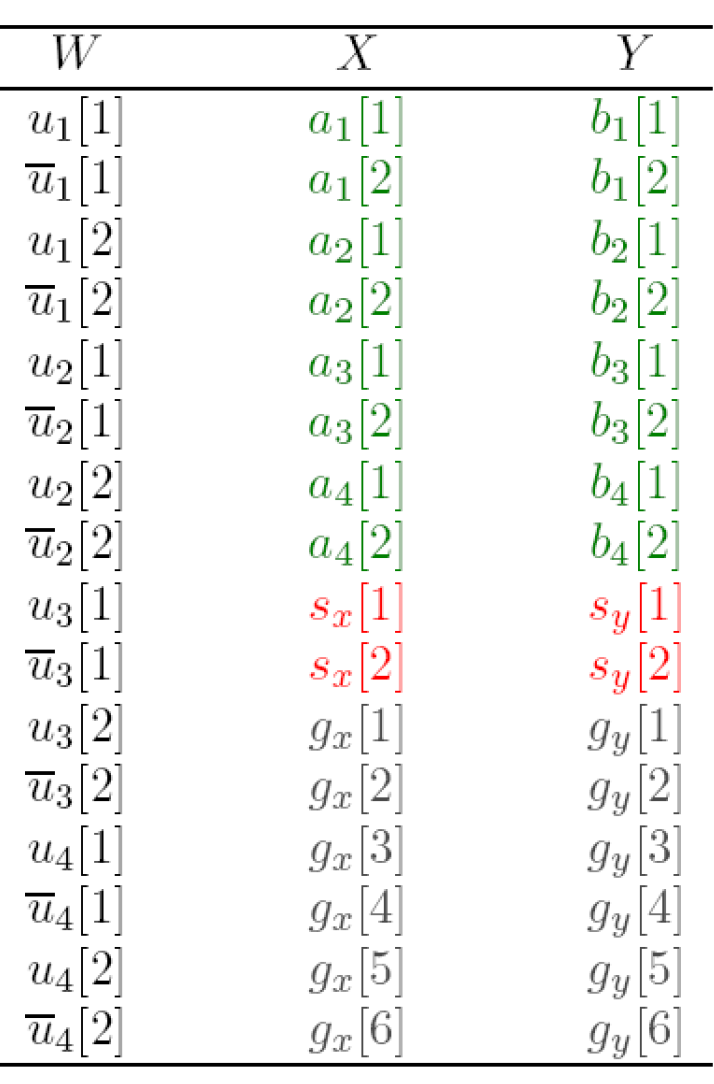
\includegraphics[width=0.5\textwidth]{photos/ejemplo_x_y_w_n_4_m_2.png}
    \caption{ $n=4$ y $m=2$}
    \label{fig:etiqueta}
\end{figure}

Se puede observar que las ternas resultantes $M$ son el producto cartesiano de $W \times X \times Y$

Esta es la forma de definir las ternas desde su definición en términos de una instancia $(U,C)$ de 3-SAT 
además $M$ se construye en tiempo polinomial

\section{Demostración $\exists M^{'} \subseteq M \Leftrightarrow (U,C) $ es satisfacible}

\subsection{$(U,C)$ satisfacible $\implies$ $M^{'} \subseteq M \Leftrightarrow$ es un matching }
Sea $t:U\rightarrow \{T,F\}$ el dominio de los valores en $U$ que satisfacen las cláusulas $C$
Para ello se construye un matching $M^{'} \subseteq M $ donde:
\begin{enumerate}
    \item Para cada cláusula $c_j \in C$: $Z_j \in \{u_i \lnot u_i: 1\leq i \leq n \}\cap c_j $
    \item Construyendo $M' = \bigcup_{t(u_i) = T} T^t_i \cup \bigcup_{t(u_i) = F} T^f_i \cup \left( \bigcup_{j=1}^{m} \{ (Z_j[j], S_x[j], S_y[j]) \} \right)$
  
Ahora definamos $G^{'}$ conjunto de m(n-1) ternas de $G$ las incluyen todos los $g_x[k] \in X , g_y[k] \ in Y$
y los $u_i[j], \lnot u_i[j] \in W$ que no se han emparejado.

Es fácil de verificar que siempre se puede construir un $G^{'}$ para que el resultado del conjunto $M^{'}$
sea una matching.

\end{enumerate}

\subsection{$M^{'} \subseteq M \Leftrightarrow$ es un matching $\implies$ $(U,C)$ satisfacible $\implies$ }
Se ha visto que para cada $u_i \in U$ $M^{'}$ incluía exactamente $m$ ternas de $T_i:$ $T^{t}_i$ o $T^{f}_i$.
Ahora, sea $t \rightarrow \{T,F\}$ donde $t(u_i)=T\leftrightarrow  M^{'} \cap T_i=T^{t}_i$  donde $t$ será una asignación correcta
que satisface a $C$.
Consideremos ahora una cláusula cualquiera $c_j \in C$, para cubrir todos los elementos internos de la componente $C_j$(de la componente de satisfacción)
Necesitamos al menos una terna de $C_j$ contenida en $M^{'}$, esta terna contiene un literal $c_j \in C$ que no estará en
$M^{'} \cap T_i$.
Además como $t(u_i)=T\leftrightarrow  M^{'} \cap T_i=T^{t}_i$ entonces $t$ satisface la cláusula $c_j$ y como todas las cláusulas $c_j \in C$
se satisfacen $(U,C)$ es satisfacible. Se cumplen los pasos previstos entonces 3-DM es NP-Completo


\end{document}








